\documentclass[11pt]{standalone}
\usepackage{amssymb}
\usepackage{amsmath}
\usepackage[no-math]{fontspec}
\usepackage{unicode-math}
\usepackage{libertinus}
\usepackage{pgf,xcolor}
\usepackage{tikz}
\usetikzlibrary{arrows.meta, backgrounds}
\usepackage{pgfplots}
\pgfplotsset{compat=newest}

\setmainfont{Libertinus Serif}
\setmathfont{Libertinus Math}

\definecolor{my_darkgray}{HTML}{484949}
\definecolor{my_lightgray}{HTML}{F3F4F4}
\definecolor{my_darkblue}{HTML}{005A94}
\definecolor{my_lightblue}{HTML}{CCDEE9}
\definecolor{my_yellow}{HTML}{FFEC7F}
\definecolor{my_red}{HTML}{E60000}
\definecolor{my_orange}{HTML}{E87846}

\begin{document}

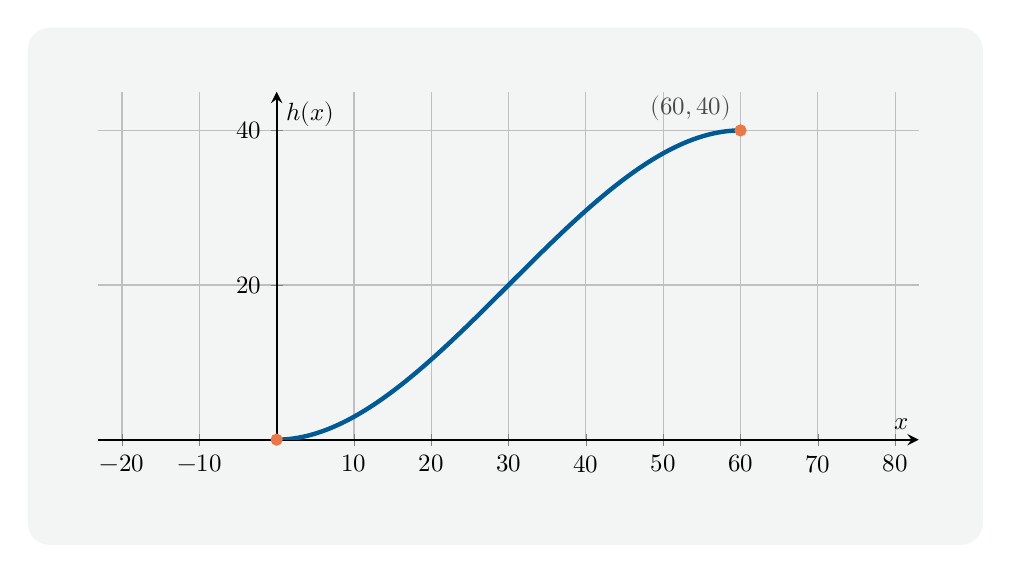
\begin{tikzpicture}[
    show background rectangle,
    background rectangle/.style={fill=my_lightgray, rounded corners=8pt},
    inner frame sep=0.8cm
]

\begin{axis}[
    width=12cm,
    height=6cm,
    axis lines = center,
    xlabel = {$x$},
    ylabel = {$h(x)$},
    xmin=0, xmax=60,
    ymin=0, ymax=45,
    grid = both,
    axis equal,
    axis line style={thick},
    ticklabel style={font=\small},
    label style={font=\small},
]

% lift hill profile h(x) = x^2/30 - x^3/2700 on [0, 60]
\addplot[
    draw=my_darkblue,
    ultra thick,
    samples=300,
    domain=0:60
]
{0.0333333333*x^2 - 0.00037037037*x^3};

% mark the base (0, 0)
\addplot[
    only marks,
    mark=*,
    mark size=2pt,
    draw=my_orange,
    fill=my_orange
]
coordinates {(0,0)};

\node[anchor=north west, font=\small, my_darkgray]
at (axis cs:0,0) {$\,(0, 0)$};

% mark the summit (60, 40)
\addplot[
    only marks,
    mark=*,
    mark size=2pt,
    draw=my_orange,
    fill=my_orange
]
coordinates {(60,40)};

\node[anchor=south east, font=\small, my_darkgray]
at (axis cs:60,40) {$(60, 40)$};

\node[anchor=south west, font=\small\bfseries, my_darkgray]
at (rel axis cs:0.02,0.98)
{Lift hill height profile $h(x) = \dfrac{1}{30}x^2 - \dfrac{1}{2700}x^3$};

\end{axis}

\end{tikzpicture}

\end{document}